\chapter{Evaluation}
\label{cha:evaluation}
In this chapter, the evaluation of the implemented prototype is presented. First, the different evaluation metrics and experiments are discussed. Then, the test dataset is described. Finally, the experiments and their results are analyzed.

\section{Evaluation metrics}
Two main factors are taken into consideration for evaluating the prototype: the quality of the clusters, which directly translates into the quality of the personas; and the performance.

\subsection{Quality of clusters}
With quality of a cluster we mean how coherent a cluster, both within itself (\textit{are the users of a cluster similar?}) and with all the users that were clustered (\textit{if there are football players among them, a cluster of sports enthusiast should be expected}). This depends on the number of clusters chosen a priori, on the distance metric and on the minimum number of activities that are collected for each user. The number of activities is relevant because, if it is too low, the chance of users' interests being misclassified in the enrichment part gets higher, since the impact of outlying activities is stronger. 

Evaluating the quality of a cluster is not an easy task, since clustering falls under the category of \textit{unsupervised learning}. This means that, usually, there is no ground truth that allows to check whether the clustering result is good or not. In fact, oftentimes the results are analyzed manually. This approach is not feasible for our fully deployed system, since the requirement of full automation would not be met. For this reason, and for the purpose of evaluation, we manually labeled our testing dataset with ground truths. This allows us to use four classic machine learning metrics, which range from 0 to 1, with 1 being the best score:
\begin{equation*}
    \begin{split}
        Accuracy = \frac{TP + TN}{TP + TN + FP + FN}
    \end{split}
    \quad
    \begin{split}
        Precision = \frac{TP}{TP + FP}
    \end{split}
    \quad
    \begin{split}
        Recall = \frac{TP}{TP + FN}
    \end{split}
\end{equation*}
where TP means \textit{true positives}, TN \textit{true negatives}, FP \textit{false positives} and FN \textit{false negatives}.
\subsection{Performance}
For performance, relevant metrics are the average time needed to enrich a single source or a single activity, as well as the total time needed for the entire process of generating personas from a collection of users.

\section{Test dataset}
The test dataset was built manually in order to have accurate ground truths. For this reason, and due to time constraints (further enforced by the APIs rate limitations), it is only composed of 90 users.

Those 90 users are all public figures who have a profile on Twitter, and were chosen in the following way: 30 football players, 30 politicians and 30 musicians/singers. These categories can be mapped to the interests classified by our system: respectively, \textit{sports}, \textit{politics} and \textit{music}. Of course, not every tweet of a politician is about politic. This was taken into account during the creation of the dataset, and only users who mainly tweeted about their respective categories were chosen.

As mentioned previously, each user is assigned a ground truth: their gender, their age bracket and their main field of interest (sports, politics, music).

\section{Experiments setup}
We have identified a set of tests, in order to evaluate the key features of the prototype. They are shown in Table \ref{table:experiments}.

In \texttt{Test1} and \texttt{Test2}, the time it takes to enrich activities and data sources is computed. \texttt{Test3} is the most important test, in which the quality of the clusters is computed and the effects of parameters like the distance metric, the number of clusters and the number of activities per user are analyzed.

\begin{table}[h]
\centering
\begin{tabular}{|c|c|c|}
    \hline
    & \textbf{Operation} & \textbf{\# of activities per user} \\
    \hline
    Test1 & Activities enrichment & [20, 50, 100] \\
    \hline
    Test2 & Data sources enrichment & [20, 50, 100] \\
    \hline
    Test3 & Clustering & [20, 50, 100] \\
    \hline
\end{tabular}
\caption{Experiments}
\label{table:experiments}
\end{table}

Other tests, for example, to evaluate the quality of the individual classifiers used in the enrichment process, are left out due to time constraints.

\section{Evaluation results}

\subsection{Activities enrichment}
The results are shown in Table \ref{table:activity_time}. As expected, the time to enrich a single activity is more or less constant. It is computed as the time difference between the reception of the activity on the enrichment queue and the moment the enriched activity is saved in the database. This average is, as expected, not influenced by the number of activities collected per user, since each enrichment is independent from the others. It is only influenced by the external API call and the time it takes to save the enrichments in the database.

The total time to enrich a given number of activities for each of the 90 users is not simply the number of total activities multiplied by the time it takes to enrich a single activity. This is caused by the quality of service setting of the pub/sub queue: by having it set to one, more time is required since the messages needs to be acknowledged before they can be processed. We have not tried setting it to zero, since some queue clients seem to disconnect at times, and that would mean losing all the messages that are sent while a client is offline. It is worth noting how, in order to collect 100 activities, the system needs to wait an entire day; this is because of the activity enrichment API, which allows at most 4500 activities to be fully enriched per day.

\begin{table}[h]
\centering
\begin{tabular}{|c|c|}
    \hline
    \textbf{Operation} & \textbf{Elapsed time} \\
    \hline
    Single activity & 0.52 seconds (average) \\
    \hline
    20 activities per 90 users & 16 minutes \\
    \hline
    50 activities per 90 users & 36 minutes \\
    \hline
    100 activities per 90 users & 75 minutes + 24h wait \\
    \hline
\end{tabular}
\caption{Performance results for activity enrichment}
\label{table:activity_time}
\end{table}

\subsection{Data sources enrichment}
The time to enrich a single data source sits at an average of 13,5 seconds, and is dominated by the interests classifier. As expected, the total time to enrich a data source is practically not affected by the number of activities per user, since the only thing that changes is the number of activities that need to be retrieved from the database. The total time to enrich 90 users is around 20 minutes.

\subsection{Clustering}
\subsubsection{Distance metric}
The distance metric used for clustering is specified in Section \ref{subsec:distance_metric}. The only parameters that needed tuning are the weights assigned to each feature. The weights were tuned in order to maximize the quality of the clusters that are presented in the following sections. Furthermore, a lot of importance was given mostly to interests, followed by gender, based on the fact that interests are the most relevant behavioral attributes available in our case for defining personas. The weights are the following:
\begin{gather*}
    Gender = 0.5 \quad Age = 0.5 \quad Language = 0.3 \quad Interests = 13 \quad Attitude = 0.3
\end{gather*}
While the weight for interests may seem high, based on tuning and experiments we conducted, it only begins to suppress the other weights around the value 100. If lowered, the gender feature tends to dominate, resulting most of the times in only two clusters, one for males and one for females.

\subsubsection{Number of clusters and activities per user}
Figure \ref{fig:silhuette} shows the silhuette score for various number of clusters and for the three different values of activities per user. It is clear that going from 20 to 50 activities per user helps narrow down the main interests of a user, thus reducing the optimal number of clusters from ten to four. Going from 50 to 100 activities does not change much, so we chose 50 as the optimal number of activities per user, which also avoids having to wait one day due to API rate limitations.

Why this happens is that, if only a small number of activities are analyzed, the risk of misclassifying a user’s interests is high. For example, during the period when our dataset was created, many Italian users tweeted about the UEFA European Football Championship, even politicians and singers. One way to avoid classifying users based on outlying activities is to simply increase the number of activities per user, thus decreasing the impact of outliers. A more sophisticated approach would consist in keeping track of what the users talk about over time, for example, month by month. This way, interests that are present only for a limited amount of time could be classified as outliers, and left out of the overall interests of the user.

\begin{figure}[h]
\centering
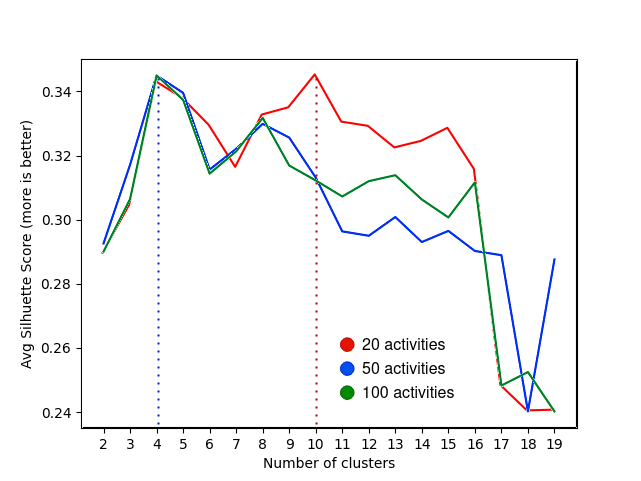
\includegraphics[width=0.65\textwidth]{img/Silhuette.png}
\caption{Silhuette score for each number of clusters, for different values of activities per user}
\label{fig:silhuette}
\end{figure}

\subsubsection{Composition of each cluster}
At this point, we analyzed how each cluster is composed. Table \ref{table:repr_users} shows the representative users, and we assigned a name to every cluster based on them. Table \ref{table:summary_clusters} shows data that can be used for computing precision, recall and accuracy.

At first glance, the results seem to be coherent with the ground truth. Two things should be noted: the first is that only musicians were split in two clusters based on gender (while the other categories are left with mixed genders); the second is that all of the representative users have \emph{culture} as their second main interest. This last observation probably happens due to the very general scope of a category such as culture. This issue could be solved by using more specialized interests classifiers, which could be chosen as a parameter by the user in order to obtain more accurate results for a specific sector (e.g. there could be one classifier specialized for the music industry, one for sports, one for food etc.). Another approach to solve it would be to ignore a specific interest if it shows up in the majority of the clusters.

\begin{table}[]
\centering
\begin{tabular}{|c|c|c|c|c|c|}
    \hline
    \textbf{Cluster} & \textbf{Gender} & \textbf{Age} & \textbf{Pref. lang.} & \textbf{Top 2 interests} & \textbf{Attitude} \\
    \hline
    1, Politicians & male & $\geq 40$ & it & Politics (0.35), Culture (0.16) & 0.02 \\
    \hline
    2, Musicians (F) & female & 19-29 & en & Music (0.26), Culture (0.10) & 0.36 \\
    \hline
    3, Musicians (M) & male & $\geq 40$ & en & Music (0.49), Culture (0.16) & 0.13 \\
    \hline
    4, Footballers & male & 30-39 & it & Sports (0.62), Culture (0.08) & 0.12 \\
    \hline
\end{tabular}
\caption{Representative users of each cluster}
\label{table:repr_users}
\end{table}

\begin{table}[]
\centering
\begin{tabular}{|c|c|c|c|c|c|}
    \hline
    \textbf{Cluster} & \textbf{\# of users} & \textbf{\# of expected users} & \textbf{TP} & \textbf{FP} & \textbf{FN}\\
    \hline
    1, Politicians & 31 & 30 & 29 & 2 & 1\\
    \hline
    2, Musicians (F) & 17 & 15 & 15 & 2 & 0 \\
    \hline
    3, Musicians (M) & 13 & 15 & 13 & 0 & 2 \\
    \hline
    4, Footballers & 29 & 30 & 29 & 0 & 1 \\
    \hline
\end{tabular}
\caption{Summary of the contents of each cluster}
\label{table:summary_clusters}
\end{table}

With this data, we can compute the metrics introduced earlier in this chapter to assess the quality of the clusters: they are shown in Table \ref{table:results}.

\begin{table}[h]
\centering
\begin{tabular}{|c|c|c|c|}
    \hline
    \textbf{Cluster} & \textbf{Accuracy} & \textbf{Precision} & \textbf{Recall} \\
    \hline
    1, Politicians & 0.96 & 0.93 & 0.96 \\
    \hline
    2, Musicians (F) & 0.97 & 0.88 & 1.0 \\
    \hline
    3, Musicians (M) & 0.97 & 1.0 & 0.86 \\
    \hline
    4, Footballers & 0.98 & 1.0 & 0.96 \\
    \hline
    Global (average) & 0.97 & 0.95 & 0.94 \\
    \hline
\end{tabular}
\caption{Results of clustering}
\label{table:results}
\end{table}

While the results are very positive, it should be noted that there is the possibility of \emph{overfitting}: that means that the system performs well on this specific test dataset, but does not generalize enough to perform well on other datasets. The only way to find out if this is the case is to try to evaluate the system with other datasets, for example by adding other categories of users. This is left out of this thesis due to time constraints.

\subsection{Final considerations}
The results of the clustering evaluation directly reflect the quality of the personas. In fact, almost all users in our dataset fall under a cluster that represents them, and the clusters themselves are meaningful and can be given an identity.

As for evaluating the personas themselves, this is still an open issue that is currently being researched. This is the case because there currently are no ways to algorithmically (thus, automatically) evaluate the quality of a persona profile; the current, most employed solution simply consists in handing out the personas to a marketing specialist, who is able to judge whether they could be useful for defining marketing strategies and choices. Again, this part is not covered in this thesis due to time constraints.